\chapter{R3 Corda Primer}
\label{chap:corda-analysis}

This chapter is meant as a short primer on Corda to better understand its architecture and functionalities in preparation for the prototype implementation details.

\section{Principal features}

Corda provides a framework specialized for use with regulated financial institutions. It is a distributed ledger system inspired by blockchains, but its design set it apart from traditional blockchain architectures.

Its main features, extracted from the \cite{cordawhitepaper} are:

\begin{enumerate}
    \item Recording and managing the evolution of financial agreements and other
    shared data between two or more identifiable parties in a way that is grounded in existing legal constructs and compatible with existing and emerging regulation
    \item Choreographing workflow between firms without a central controller.
    \item Supporting consensus between firms at the level of individual deals, not a
    global system.
    \item Supporting the inclusion of regulatory and supervisory observer nodes.
    \item Validating transactions solely between parties to the transaction.
    \item Supporting a variety of consensus mechanisms.
    \item Recording explicit links between human-language legal prose documents and smart contract code.
    \item Using industry-standard tools.
    \item Restricting access to the data within an agreement to only those explicitly entitled or logically privileged to it.
\end{enumerate}

\section{Network topology}

A Corda network is made up of authenticated nodes engaging in peer-to-peer communication, where each node is a Java Virtual Machine runtime hosting Corda services and executing CorDapps. All comunication is direct and TLS-encrypted: the data is shared only on a need-to-know basis between nodes, and there are no global broadcasts.

A Corda network has a figure known as the doorman. Such service enforces identification at network entry and based on the rules it was set up with, admits nodes to the network - this is what makes Corda a permissioned, private distributed ledger.

Identities in Corda are certificates (X.509) which represent the legal identity of an organisation or service identity of a network service.

\section{Core mechanics}

In Corda there's no single central store of data. Instead each node mantains a separate database of states. The entirety of the distributed ledger is made up of the union of such databases - which are called vaults. The union of states strictly regarding a transaction between two nodes makes up the ledger between two nodes.

States are what are recorded on ledgers, and represent facts such as funds possessed by the node's owner, loans, or any kind of financial agreement between parties. States are immutable and evolve. A state consumed by a transaction becomes historic, and can be replaced by a new state generated by the same transaction.

Transactions are regulated by contracts: a contract verifies if a transaction abides by its rules, and if it does, is verified and can be finalized in the ledgers of the parties engaging in it. Transactions take in a set of input states and generate a set of output states. Transaction validity is given by the digital signatures of the parties engaging in it and the smart contract itself. 

Consensus is computed through a third node, the Notary, which attests that for a given transaction it has not already signed other transactions that consumes any of the proposed transaction's input states - thus preventing double-spends.
As the consensus is pluggable in Corda, any of the given algorithms can be used for computing the consensus. 
Furthermore, every input state is walked through its history, to verify if every state that brought to the final and current one is valid - this is called validity consensus.

Flows are automatization of transactions. The flow framework allows developers to automate the process rather than specify the transaction steps manually. Nodes in Corda are made to communicate through flows.
\newpage

\section{CorDapp}

CorDapps are distributed applications running on the Corda platform, allwoing nodes to communicate. This is achieved by defining flows that Corda node owners can invoke through RPC calls or HTTP APIs.

CorDapp in Corda can be written either in Java or Kotlin. And their main components are:

\begin{enumerate}
    \item State classes, defining the facts over which agreement is reached
    \item Contract classes, defining what constitutes a valid ledger update 
    \item Flow classes, defining flows for transactions
\end{enumerate}

Between other components, we list Serialization whitelists classes, which restrict what types a node can receive off the wire, and Service subclasses that provide long-lived utilites within the node.

\begin{figure}[b]
    \centering
    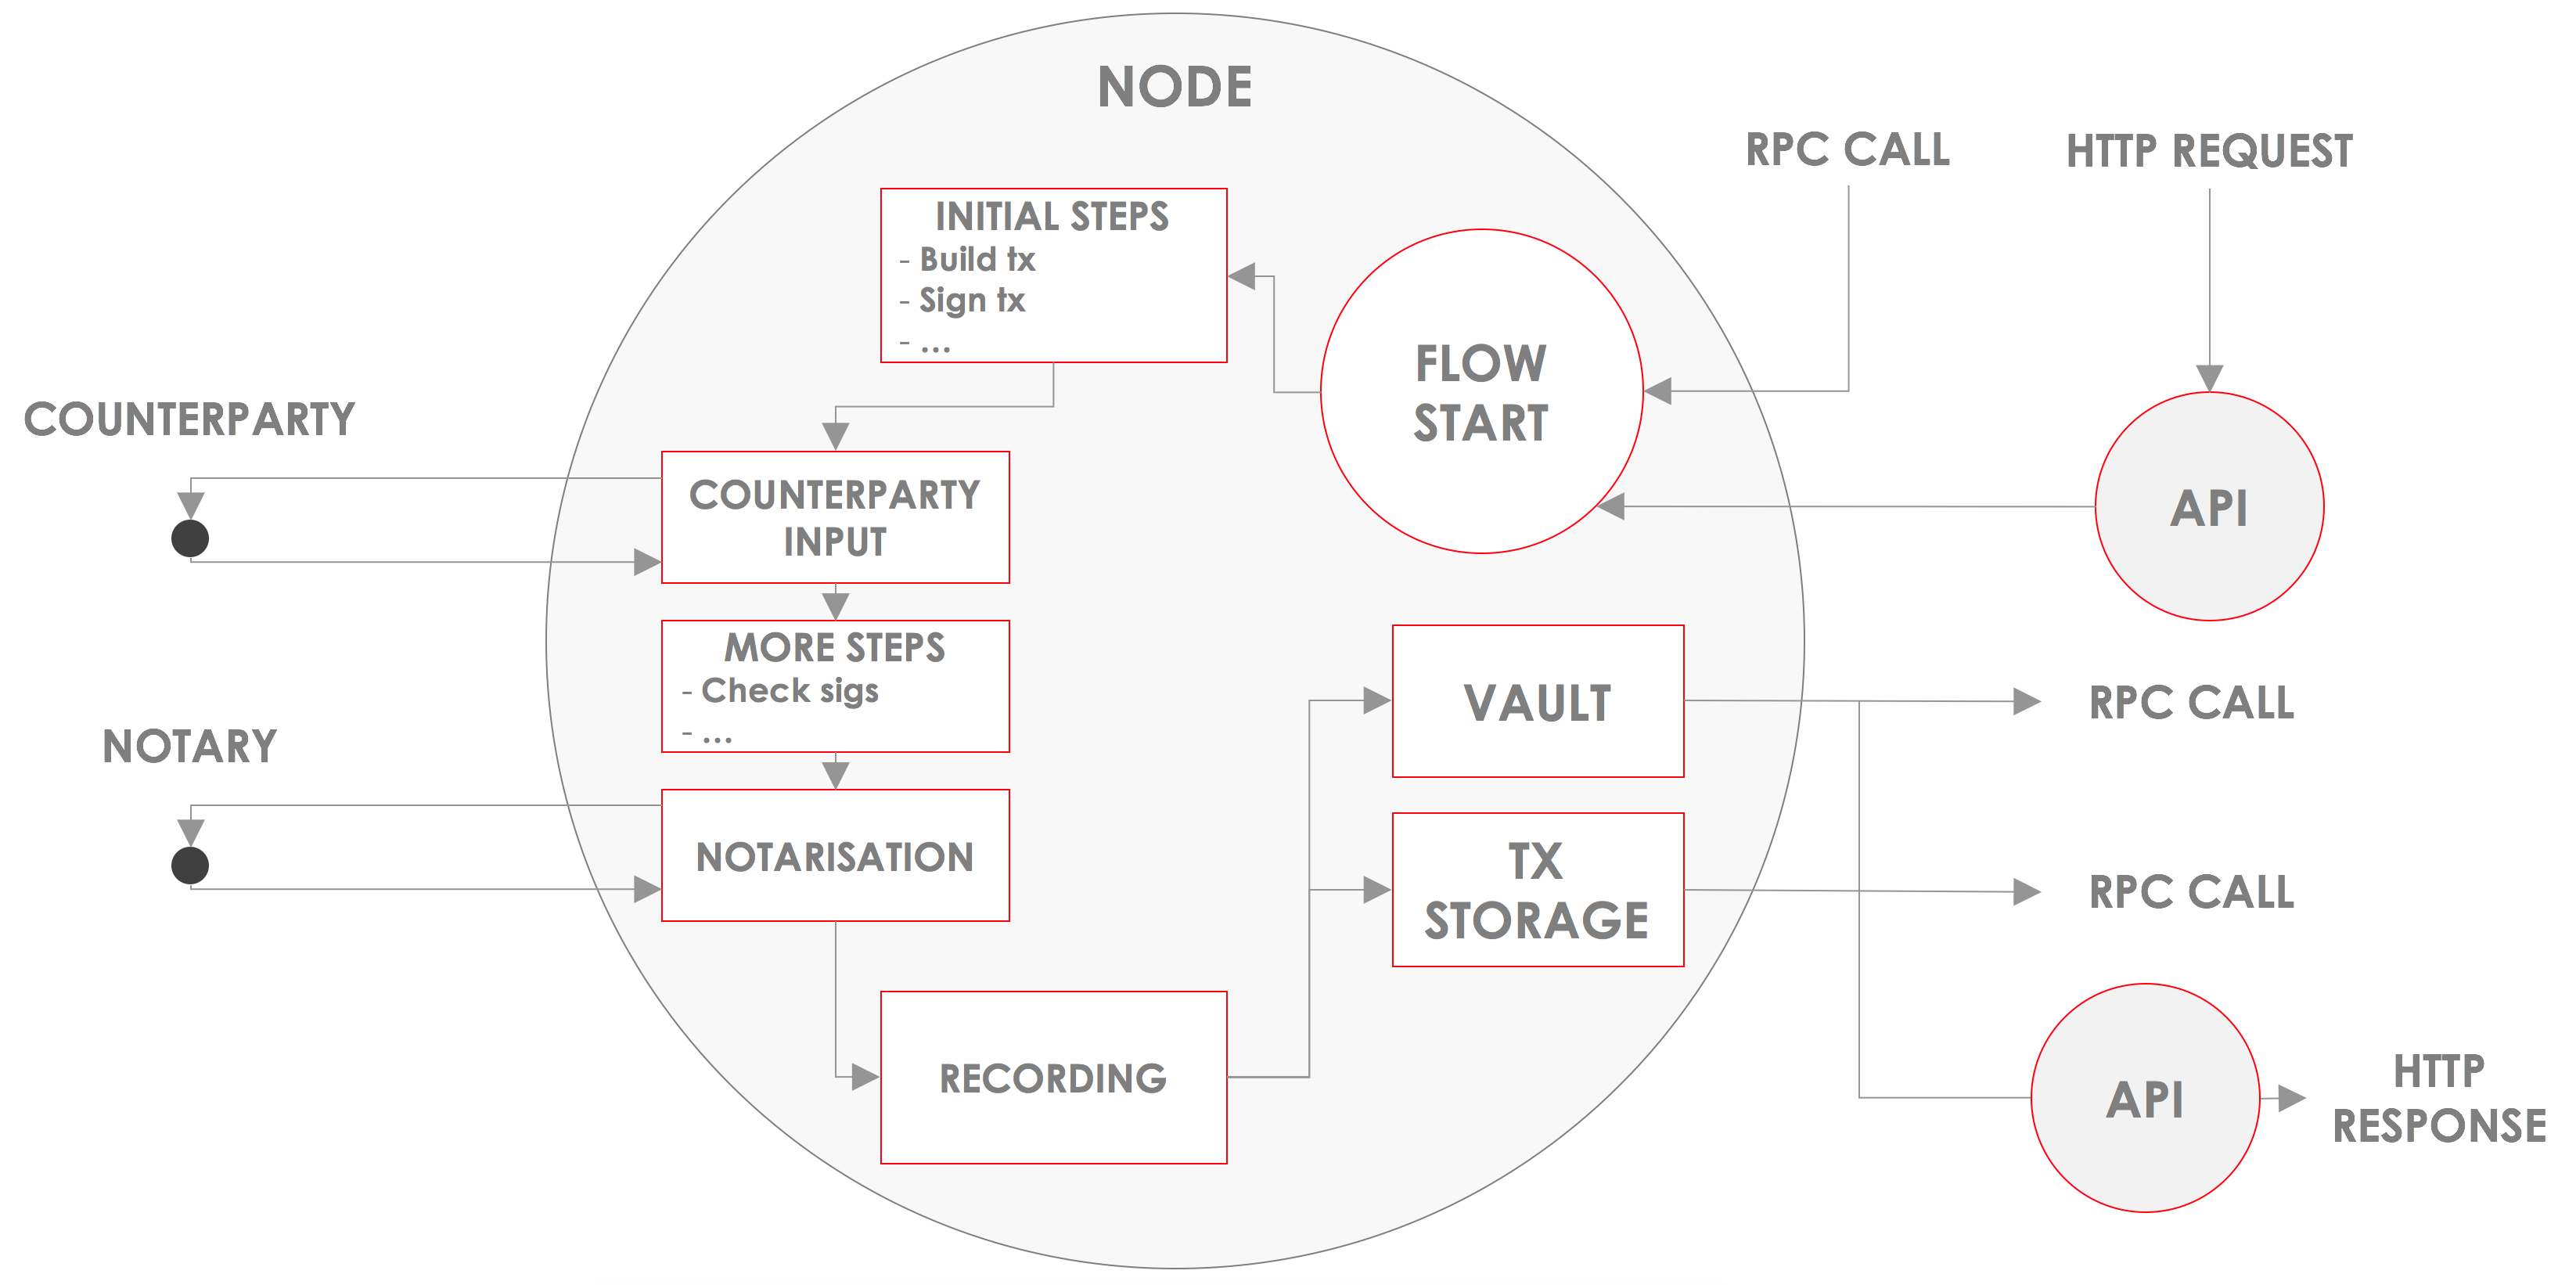
\includegraphics[scale=0.2]{cordapp.png}
    \caption{CorDapp structure diagram}
\end{figure}

